\documentclass[conference]{IEEEtran}
% \IEEEoverridecommandlockouts
% The preceding line is only needed to identify funding in the first footnote. If that is unneeded, please comment it out.
\usepackage{cite}
\usepackage{amsmath,amssymb,amsfonts}
%\usepackage{algorithmic}
\usepackage{graphicx}
\usepackage{textcomp}
\usepackage{xcolor}
%\usepackage{hyperref}
\include{~/template/packages.tex}
\def\BibTeX{{\rm B\kern-.05em{\sc i\kern-.025em b}\kern-.08em
    T\kern-.1667em\lower.7ex\hbox{E}\kern-.125emX}}
\begin{document}

\title{CS 6375 Assignment 1 \\
\href{github.com/...}{github.com/...}
}

\author{\IEEEauthorblockN{Nathan J. Whitehead}
\IEEEauthorblockA{\textit{University of Texas at Dallas}\\
nathan.whitehead@utdallas.edu \\
njw240000 \\
}
% \and
% \IEEEauthorblockN{2\textsuperscript{nd} Given Name Surname}
% \IEEEauthorblockA{\textit{dept. name of organization (of Aff.)} \\
% \textit{name of organization (of Aff.)}\\
% City, Country \\
% email address or ORCID}
% \and
}

\maketitle


\section{Introduction and Data (5pts)}

The goal of this assignment is to implement a sentiment classifier on a dataset of yelp reviews, which are labeled with a sentiment level of 1-5. The dataset is split into a training set, a validation set, and a test set the classifier model is trained on the training and validation sets, then evaluated on the test set. There were two architectures of neural networks used: a simple feedforward neural network and a recurrent neural network. The recurrent neural network also made use of a word embedding layer. The performance of the two models was tuned and evaluated. 
The final RNN product was able to classify the sentiment of the reviews with an accuracy of 0.4, which is better than random guessing, but not particularly impressive. 
The FFNN was only able to achieve an accuracy of 0.33, which is equivalent to random guessing.

\subsection{Data} 

The data includes 17,600 reviews, with 16,000 in the training set, 800 in the validation set, and 800 in the test set. 

% Training distribution: {'1': 3200, '2': 3200, '3': 3200, '4': 3200, '5': 3200}
% Validation distribution: {'1': 320, '2': 320, '3': 160, '4': 0, '5': 0}
% Test distribution: {'1': 0, '2': 0, '3': 160, '4': 320, '5': 320}

\begin{table}[htbp]
\caption{Data Overview}
\begin{center}
\begin{tabular}{cccccc}
\hline
\textbf{Sentiment} & \textbf{1} & \textbf{2} & \textbf{3} & \textbf{4} & \textbf{5} \\
\hline
Training & 3200 & 3200 & 3200 & 3200 & 3200 \\
Validation & 320 & 320 & 160 & 0 & 0 \\
Testing & 0 & 0 & 160 & 320 & 320 \\
\hline
Total & 3520 & 3520 & 3680 & 3520 & 3520 \\
\end{tabular}
\end{center}
\label{default}
\end{table}%

\section{Implementations (45pts)}

\subsection{Feedforward Neural Network (20pts)}

The incomplete code for the FFNN was completed as follows: 

\subsubsection{Forward}

The \texttt{forward()} function was completed by implmenting the forward pass of the FFNN. When given an input vector, it computes the hidden layer representation, then the output layer representation, and finally the probability distribution of the output, i.e. the predicted vector. The input vector is first passed through the first weight matrix $W_1$, followed by the activation function, which introduces non-linearity to the model (line 3). The transformed hidden layer is then passed through the second weight matrix $W_2$ to obtain the raw output logits (line 5). Finally, the output layer representation is passed through the softmax function to convert the raw logits to a predicted probablility distribution over the classes (line 7).

\begin{lstlisting}[language=Python]
def forward(self, input_vector):
  # [to fill] obtain first hidden layer representation
  hidden = self.activation(self.W1(input_vector))
  # [to fill] obtain output layer representation
  output = self.W2(hidden)
  # [to fill] obtain probability dist.
  predicted_vector = self.softmax(output)
  return predicted_vector
\end{lstlisting}

\subsubsection{Other Code additions}

There were a few other code modifications that were made to the FFNN. 

First, the \texttt{load\_data()} function was modified to add the 
capability for including test data, and to verify the scope of the data 
provided.

\begin{lstlisting}[language=Python]
def load_data(train_data, val_data, test_data=None):
  train_stars = {"1": 0, "2": 0, "3": 0, "4": 0, "5": 0}
  with open(train_data) as training_f:
    training = json.load(training_f)
    for line in training:
      train_stars[str(int(line["stars"]))] += 1
  print(f"Training distribution: {train_stars}")

  val_stars = {"1": 0, "2": 0, "3": 0, "4": 0, "5": 0}
  with open(val_data) as valid_f:
    validation = json.load(valid_f)
    for line in validation:
      val_stars[str(int(line["stars"]))] += 1
  print(f"Validation distribution: {val_stars}")

  test_stars = {"1": 0, "2": 0, "3": 0, "4": 0, "5": 0}
  if test_data:
    with open(test_data) as test_f:
      test = json.load(test_f)
      for line in test:
        test_stars[str(int(line["stars"]))] += 1
    print(f"Test distribution: {test_stars}")

  tra = []
  val = []
  tst = []
  for elt in training:
    tra.append((elt["text"].split(), int(elt["stars"] - 1)))
  for elt in validation:
    val.append((elt["text"].split(), int(elt["stars"] - 1)))
  for elt in test:
    tst.append((elt["text"].split(), int(elt["stars"] - 1)))

  return tra, val, tst
\end{lstlisting}

The testing section in the \texttt{main()} function was added to 
allow the user to test the model on the test data. 

\begin{lstlisting}[language=Python]
  # now test the model
  if args.do_train:
    print("========== Testing =========")
    model.eval()
    correct = 0
    total = 0
    start_time = time.time()
    print("Testing started")
    minibatch_size = 16
    N = len(test_data)
    for minibatch_index in tqdm(range(N // minibatch_size)):
      optimizer.zero_grad()
      loss = None
      for minibatch_index in tqdm(range(N // minibatch_size)):
        optimizer.zero_grad()
        loss = None
        for example_index in range(minibatch_size):
          input_vector, gold_label = test_data[minibatch_index * minibatch_size +
                                               example_index]
          predicted_vector = model(input_vector)
          predicted_label = torch.argmax(predicted_vector)
          correct += int(predicted_label == gold_label)
          total += 1
          example_loss = model.compute_Loss(
            predicted_vector.view(1, -1), torch.tensor([gold_label])
          )
          if loss is None:
            loss = example_loss
          else:
            loss += example_loss
        loss = loss / minibatch_size

    print("Testing completed")
    test_accuracy = correct / total if total > 0 else 0
    print("Testing accuracy: {}".format(test_accuracy))
    print(f"Testing time: {(time.time() - start_time):.2f}")
\end{lstlisting}

There were also various other code modifications made to the \texttt{main()}
function, including adding a few timers to measure the time taken for training at each step, and a few variables such as \texttt{test\_accuracy} to store various metrics, which are then output to a file at the end of testing.

\subsubsection{Other parts of the code}

The rest of the code is the same as the provided template for the assignment. 
To briefly summarize, the code begins by defining the FFNN class, which is a subclass of the torch.nn.Module class. The FFNN class has a constructor that initializes the hidden dimensions $h$, the two weight matrices $W_1$ (maps the input vector to a hidden layer of size $h$) and $W_2$, (maps a hidden layer to the output space of size 3), and the softmax and loss functions, which are used to compute the output probability distribution and the loss, respectively. The class also has a \texttt{forward()} function, explained above.

The program begins by loading the user arguments, loading the data, and converting the data to a vector representation. The model is then inizialized and the stochastic gradient descent optimizer is initialized with a learning rate of 0.01 and momentum of 0.9. This contols how much the model weights are updated at each step and accelerates the learning to avoid oscillation. Then, the model is trained on the training and validation data in epochs, where each epoch is a full pass through the training data. The model is evaluated on the validation data at each epoch, and the model with the best validation accuracy is saved. This continues for a set number of epochs defined by the user. In my case, I used 10 epochs.

Finally, the model is tested on the test data, and the accuracy is output to the user and saved to a file. The best accuracy I was able to achieve was 0.xxx.


\subsection{Recurrent Neural Network (25pts)}

The incomplete code of the RNN was completed as follows:

\subsubsection{Forward}

The forward function of the model was completed by first passing the input sequence through the RNN layer, retrieving the hidden states of the RNN at each step (\texttt{output}), and the final hidden state of the RNN (\texttt{hidden}). Then the output of the RNN is summed over the sequence dimension to aggregate information from all time steps into a single vector (\texttt{summed\_output}). This vector is then passed through the weight matrix \texttt{W} to obtain the raw output logits (\texttt{logits}). Finally, the raw logits are passed through the softmax function to obtain the predicted probability distribution over the classes (\texttt{predicted\_vector}).

\begin{lstlisting}[language=Python]
def forward(self, inputs):
  # option b:
  output, hidden = self.rnn(inputs)  
  summed_output = output.sum(dim=0)  
  logits = self.W(summed_output)  
  predicted_vector = torch.nn.functional.softmax(
    logits, dim=-1
  ) 
  return predicted_vector
\end{lstlisting}

\subsubsection{Other Code additions}

Similar code modifications to normalize testing data and add testing functionality were made as in FFNN above. The output file was also added to maintain results. A conditional was also added to the training loop to allow the model to complete training when the user-specified number of epochs is reached.

\subsubsection{Other parts of the code}

The rest of the code is the same as the provided template for the assignment. The model is defined as a subclass of the torch.nn.Module class, with a constructor that initializes the RNN layer, the weight matrix, the softmax function, and the loss function. The forward function is defined as above. 

The program begins by loading the user arguments, loading the data, and converting the data to a vector representation based on the word embeddings provided.

Then the model is trained in epochs, similarly to the FFNN, but with the added condition that the model will stop training early if the validation accuracy reduces while training accuracy increases, to avoid overfitting. The model is evaluated on the validation data at each epoch, and the model with the best validation accuracy is saved. This continues for a set number of epochs defined by the user. In my case, I used 10 epochs.

Finally, the model is tested on the test data, and the accuracy is output to the user and saved to a file. The best accuracy I was able to achieve was 0.xxx.


\section{experiments and Results (45pts)}

\subsection{Evaluations (15pts)}

The models were evaluated on the test data, with the metric being used was the accuracy, defined as the number of correct predictions divided by the total number of predictions the model makes.
Given that there are five classes of outputs, the random guessing accuracy is 0.2. 
The FFNN was able to achieve an accuracy of 0.33, which is equivalent to random guessing. 
The RNN was able to achieve an accuracy of 0.4, which is only slightly better than random.

\subsection{Results (30pts)}

\begin{table}[htbp]

\caption{Results}
\begin{center}
\begin{tblr}{cccc}
\hline
\textbf{Model} & Hidden Layers & Epochs & \textbf{Accuracy} \\
\hline
{\SetCell[r=6]{c} FFNN} & 2 & 10 & 0.3975 \\
 & 4 & 10 & 0.38875 \\
 & 8 & 10 & 0.5225 \\
 & 16 & 10 & 0.49875 \\
 & 32 & 10 & 0.5 \\
 & 64 & 10 & 0.50375 \\
\hline
{\SetCell[r=6]{c}RNN} & 2 & 10 & 0.4 \\
 & 4 & 10 & 0.4 \\
 & 8 & 10 & 0.0 \\
 & 16 & 10 & 0.xx \\
 & 32 & 10 & 0.xx \\
 & 64 & 10 & 0.xx \\
\hline
\end{tblr}
\end{center}
\label{default}
\end{table}%


\section{Analysis (bonus: 10pts)}

Learning curve of the best system: FFNN with 8 hidden layers.

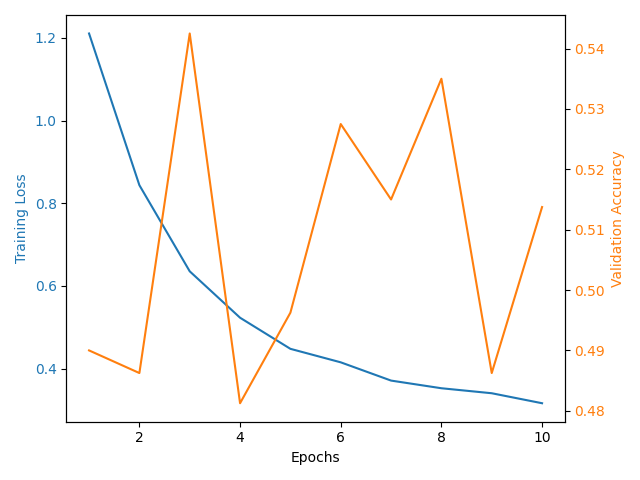
\includegraphics[width=3in]{../cs6375_2025_assignment1_release/learning_curve.png}

\section{Conclusion and Others (5pts)}

Feedback: I felt the assignment was interesting, but I would have appreciated more guidance on what was expected, for example, what the expected accuracy was. I also found some aspects confusing, such as the dataset. For the awhile I was training using a dataset that didn't contain examples for sentiments 4 and 5, which caused a lot of issues when testing. I also found some of the code confusing, it felt like there were sections extant from past assignments that were unrelated to what we were told to fill in. It is made clear that the only thing to change is the forward function, but there was no test code provided, so that obviously required more editing, which was fine, just a bit confusing.

\end{document}